\documentclass{article}
\usepackage{graphicx} 
\title{Requirements and Design Documentation}
\author{devs101}

\begin{document}
\maketitle
\tableofcontents
\newpage

\section{Functional Requirements}
The user must be able to do the following:
\begin{enumerate}
\item Add a new node to the tree. This is the most important functionality, because nodes must be added to create a tree.
\item Delete an existing node from the tree. It is important that if a user can add a node, the user should also be able to remove a node if it is no longer needed or wanted.
\item Edit the following settings of a node:
 \begin{itemize}
  \item Name. This is a String variable, it is the label of the node and the name that will be used to refer to this node.
  \item ID. This is a String variable and it must be unique, it is the nodes unique identification, it will be used by the program to retrieve this node.
  \item Description. This is a String variable, it is a custom user defined description of the node and its use.
  \item Visible. This is a boolean variable, it states whether or not the node should be display.
  \item Enabled. This is a boolean variable that is determined if all of the nodes prerequisites are met or not. This value is usually automatically set using a function, however a user can manually change it for testing purposes.
  \item Max. This is a integer variable, it states how many times this skill/node can be bought/upgraded.
  \item Cost. This is a integer variable, it states how many points is needed to acquire/upgrade this skill/node.
 \end{itemize}
 \item Links between nodes must be automatically created, but links can also be manually set and changed in the editor. This is important, because a tree is a structure of interconnected nodes. If the nodes had no links then it would not be a tree.
\item Create custom global variables that will be used in the tree structure. This allows the users to add their own data that will be used by the system.
\item The custom variables must be usable in the node settings. This is important for the users data to be used by the system, the user can use their data to change a node�s settings or provide conditions to certain settings.
\item Automatically produce a layout of the current nodes. This is important, because this determines where newly added nodes appear on the screen.
\item Move an existing node around in the tree view. This allows the user to create their own layout of the tree.
\item Zoom in and out of the tree view. This is a simple but important functionality to be able to view the tree in different ways.
\item Save and Load the state of the tree at any point in time. Save data must be stored in a JSON format. This is very important to keep track of the user's progress and keep it safe incase something happens and the site crashes that the tree and the data is not lost.
\item Undo and Redo any actions or changes performed on the tree at any point in time. Must be able to undo as many times as actions were performed, undo until original tree state is reached. This uses the previous saved states of the tree. This is useful for quickly undoing a small mistake.
\item Copy a node and all its properties. This is useful for when a user wants identical nodes or if the user wants to add a node from one tree to another tree without creating a new node from scratch.
\item Paste a copied node to the tree view. This is needed for the copying of a node. This recreates the node/nodes with all the properties that was copied. Without the paste functionality,  the copy functionality would be pointless.
\item Multi selection of nodes. Must be able to select multiple nodes at once and perform all node operations (Move, Copy, Paste, Delete, Edit, etc.) to all selected nodes at once. This is useful for when the user wishes to work in bulk.
\item Edit how the nodes, links and background looks. This is to further expand the tree�s customization. 
\end{enumerate}

The user should be able to perform tests on the skill tree and be able to:

\begin{itemize}
\item Specify global variable values and amount of skill points available. This allows users to set the initial starting values of their global variables, that they can change at any time, as well as the amount of skill points available for them to spend on the tree.
\item Buy skills with skill points. This lets the users test that the skill/node settings are working properly.
\item Reset skill points. This lets the user clear all the points that has been spent and start from the beginning. This is very useful for testing purposes.
\item Export the current tree (the current state of the tree) as a JavaScript file that web developers can use to import, display and use a skill tree on their own webpage. This gives users the ability to share their skill trees with others. If a user imports this JavaScript file the program will recreate that skill tree at the state it was saved when it was exported.
\item Allow the developer to give a skill tree json file that can set global parameters and set initial selected skills. This allows the user to use the developer of the tree�s global variables and other initial values, instead of the users own global variables and initial values. This is from importing an exported tree.
\item Allow the user to query what skills have been selected. This is to provide testing conditions for certain skills based on the values of the global variables and other settings. Example if a variable states that only skills from class A can be selected and the user tries to select a skill from class B then that skill must not be selectable.
\item Allow the users to trigger their own functions when skills are selected. This is to further expand the testing conditions for skills by allowing user defined events to occur on certain actions. Example if a user attempts to select a skill that should not be selected, a pop up will appear stating that this skill is unavailable.
\item All these functionality should be demonstrated with jsFiddle.
\end{itemize}

\section{Domain Model}

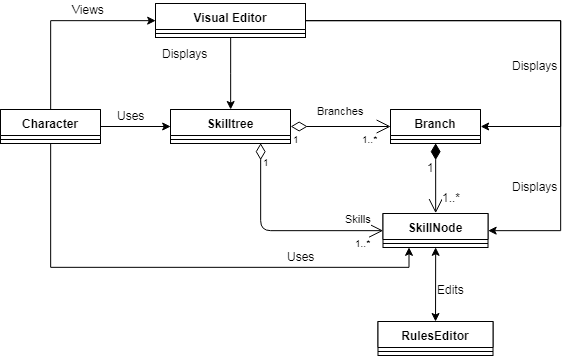
\includegraphics{TriiDomainModel}

\section{Architectural Design and Structure}

The Trii system is based on the Client-Server architecture style. This is because the website is the server that provides the service of the skill tree software to several clients that connect to the server. The clients can connect from anywhere to the server via a http protocol and use the software from their own work station. The system also makes use of the MVC architectural design that provides a display area for the user where the tree can be viewed and its layout be modified by direct input (example dragging nodes around the display area). The system also uses a editor that allows the user to change the settings of nodes and to create global variables and assign values to these variables, all that will affect the structure and interaction with the tree.

\end{document}



